\documentclass{article}
\usepackage[utf8]{inputenc}

\title{TMA4195 Mathematical Modelling Project}
\author{Group 1: 736142, 494865, 760446 ...}
\date{\today}

\usepackage[square,numbers]{natbib}
\bibliographystyle{abbrvnat}% Makes the bibliography file available to biblatex.
\usepackage{graphicx}
\usepackage{amsmath}
\usepackage{amsfonts}
\usepackage{amssymb}
\usepackage{cancel}
\usepackage{mathtools}
\usepackage{parskip}
\setlength{\parskip}{7pt}
\usepackage{mdframed}
\usepackage[hypertexnames=false,bookmarksopen=true]{hyperref}
\usepackage{xcolor}
\usepackage{float}
\hypersetup{
    colorlinks,
    linkcolor={blue!30!black},
    citecolor={blue!30!black},
    urlcolor={blue!30!black}
}
\usepackage{geometry}
\geometry{
 a4paper,
 total={160mm,240mm},
 left=25mm,
 top=25mm,
 }
 
\begin{document}
\maketitle

\section{General governing equations}
\subsection{Mass conservation equation}

Let us consider a closed region $R$ with boundary $\partial R$ in space. We have a material with density $\varphi \, (x,t)$  moving with a flux $j\, (x,t,\rho)=\varphi \vec{u}$. For the sources and sinks inside $R$ we consider a generalized production density $q\, (x,t)$. In this case, the conservation law in integral form may be written as follows,

\begin{equation}
\label{general_balance}
\dfrac{d}{dt}\int_R \varphi(x,t) \, dV + \int_{\partial R} \varphi(x,t) \vec{u}\cdot \vec{n} \, d\sigma=\int_R q(x,t) \, dV
\end{equation}
For the mass conservation, $\varphi \, (x,t)=\rho \, (x,t)$. Without sources and sinks, the mass within a material region will be constant and thus the production term will be zero, $q\, (x,t)=0$.

\begin{equation}
\dfrac{d}{dt}\int_R \rho \, dV + \int_{\partial R} \rho   \vec{u}\cdot \vec{n} \, d\sigma=0
\end{equation}
When $\rho$ and $u$ are sufficiently smooth, it is possible to differentiate under the integral sign and apply the Divergence Theorem:
\begin{align}
\label{differential}
\frac{d}{dt}\int_R \rho \, dV =& \int_R \frac{\partial \rho}{\partial t} \, dV,\\
\label{divergence}
\int_{\partial R} \rho \vec{u} \cdot n \, d\sigma =& \int_R \nabla \cdot (\rho \vec{u})\, dV
\end{align}
so that
\begin{equation}
\int_R \left( \dfrac{\partial \rho}{\partial t} + \nabla \cdot (\rho \vec{u}) \right) dV=0
\end{equation}
Let us now consider a ball $B(x,r) \subset R$ centered in $x$ with radious $r$ and take the following limit when $r \rightarrow 0$,
\begin{equation}
\label{ball}
\lim_{x \to 0} \frac{\int_{B(x,r)} \left( \dfrac{\partial \rho}{\partial t} + \nabla \cdot (\rho \vec{u}) \right) dV}{\int_{B(x,r)}dV}=0 \Rightarrow \dfrac{\partial \rho}{\partial t} + \nabla \cdot (\rho \vec{u})=0
\end{equation}
Here we get the mass conservation law in differential form:
\begin{equation}
\label{mass}
\boxed{
\dfrac{\partial \rho}{\partial t} + \nabla \cdot (\rho \vec{u})=0
}
\end{equation}
\subsection{Momentum conservation equation}

In \hyperref[general_balance]{Eq.~\ref{general_balance}}, $\varphi \, (x,t)=\rho \, (x,t) \vec{u}$, and the production term $q\, (x,t)$ is the net force acting on the mass in $R$. So that:

\begin{equation}
\dfrac{d}{dt}\int_R \rho \vec{u} \, dV + \int_{\partial R} \rho \vec{u} (\vec{u}\cdot \vec{n}) \, d\sigma=\sum F
\end{equation}

Neglecting gravity and viscous force, we only consider the pressure acting on the system. We can express this force in terms of the stress tensor $\vec{T}$ which is containing the value $-p$ in the elements of the diagonal. Taking this into account, we get:

\begin{equation}
\sum F=\int_{\partial R}\vec{T}\cdot \vec{n} \, d\sigma=\sum F=\int_{\partial R}-\vec{p}\cdot \vec{n} \, d\sigma
\end{equation}

Similarly as in \hyperref[differential]{Eq.~\ref{differential}} and \hyperref[divergence]{Eq.~\ref{divergence}}, we differentiate under the integral sign and apply the Divergence Theorem:

\begin{equation}
\int_R \left( \frac{\partial \rho \vec{u}}{\partial t} + \nabla \cdot (\rho \vec{u} \otimes \vec{u}) \right) dV=\int_R -\nabla \vec{p} \, dV
\end{equation}

Considering now a ball $B(x,r) \subset R$ centered in $x$ with radious $r$ and letting it tend to a point as in \hyperref[ball]{Eq.~\ref{ball}}, we get the momentum conservation law in differential form:


\begin{equation}
\label{momentum}
\boxed{
(\rho \vec{u})_t  + \nabla \cdot (\rho \vec{u} \otimes \vec{u})=-\nabla \vec{p}
}
\end{equation}

If we decompose \hyperref[momentum]{Eq.~\ref{momentum}} for each direction in space, we get:
\begin{eqnarray}
\label{1direction}
(\rho u_1)_t  + \nabla \cdot (\rho u_1 u)=-\frac{\partial p}{\partial x} \\
\label{2direction}
(\rho u_2)_t  + \nabla \cdot (\rho u_2 u)=-\frac{\partial p}{\partial y} \\
\label{3direction}
(\rho u_3)_t  + \nabla \cdot (\rho u_3 u)=-\frac{\partial p}{\partial z}
\end{eqnarray}

\subsection{Energy conservation equation}

The first law of Thermodynamics states that:
\begin{equation}
\label{fistlaw}
    dU = dQ + dW\Rightarrow \dfrac{dU}{dt}=\dfrac{dQ}{dt}+\dfrac{dW}{dt}\ 
\end{equation}
This notation considers the terms $dQ$ and $dW$ to be the heat supplied to the CV and the work exerted on the system, respectively. Applying the Reynolds transport theorem, the total energy $U$ is defined as:
\begin{align}
\label{energy}
\dfrac{dU}{dt}=& \dfrac{d}{dt}\int_{R(t)}u\rho\,dV\nonumber\\ =& \dfrac{d}{dt}\int_{R}u\rho\,dV + \int_{\partial R}u\rho\vec{u}\cdot\vec{n}\,d\sigma\nonumber\\
=& \dfrac{d}{dt}\int_{R}\left(\frac{|\vec{u}|^2}{2}+e\right)\rho\,dV + \int_{\partial R}\left(\frac{|\vec{u}|^2}{2}+e\right)\rho\vec{u}\cdot\vec{n}\,d\sigma
\end{align}

where $u=\frac{|\vec{u}|^2}{2}+e$ is the specific energy and $e$ the internal specific energy.

The only work acting on the CV is that from the pressure forces acting:
\begin{equation}
\label{workWs}
    \dfrac{dW}{dt}=\dfrac{dW_s}{dt}=\int_{\partial R}(T\vec{n})\cdot\vec{u}\,d\sigma=\int_{\partial R}(T\vec{u})\cdot\vec{n}\,d\sigma=\int_{\partial R}(-pI\vec{u})\cdot\vec{n}\,d\sigma=\int_{\partial R}(-p\vec{u})\cdot\vec{n}\, d\sigma
\end{equation}
We can express the heat flux going to the system following Fourier's law:
\begin{equation}
\label{fourierQ}
    \dfrac{dQ}{dt}=-\int_{\partial R}\vec{q}\vec{n}\,d\sigma=-\int_{\partial R}(-\kappa \nabla T)\vec{n}\,d\sigma=\int_{\partial R}\kappa \nabla T\vec{n}\,d\sigma
\end{equation}
Inserting {expressions~\ref{energy},~\ref{workWs} and~\ref{fourierQ}} into {Eq.~\ref{fistlaw}}:
\begin{equation}
\dfrac{d}{dt}\int_{R}\left(\frac{|\vec{u}|^2}{2}+e\right)\rho\,dV + \int_{\partial R}\left(\frac{|\vec{u}|^2}{2}+e\right)\rho\vec{u}\cdot\vec{n}\,d\sigma=\int_{\partial R}(-p\vec{u})\cdot\vec{n}\, d\sigma+\int_{\partial R}\kappa \nabla T\vec{n}\,d\sigma
\end{equation}

Similarly to the process followed in the mass and momentum balances, we apply Divergence Theorem and consider a ball in the CV region and let it tend to a point:
$$
\int_{R}\frac{\partial}{\partial t}\left(\frac{|\vec{u}|^2}{2}+e\right)\rho\,dV + \int_{R}\nabla\cdot\left(\frac{|\vec{u}|^2}{2}+e\right)\rho\vec{u}\,dV=\int_{ R}\nabla\cdot\left(\kappa \nabla T\right)\,dV+\int_{R}\nabla\cdot(-p\vec{u})\, dV \Rightarrow 
$$
\begin{equation}
\Rightarrow \left(\rho\left(e+\frac{|\vec{u}|^2}{2}\right)\right)_t + \nabla\cdot\left(\rho\vec{u}\left(e+\frac{|\vec{u}|^2}{2}+\frac{p}{\rho}\right)-\kappa\nabla T\right)=0
\end{equation}

By introducing the definition for specific enthalpy $h=e+\frac{p}{\rho}$ we get to the desired result:
\begin{equation}
    \boxed{
    (\rho(e+\frac{1}{2}|\vec{u}|^2))_t + \nabla\cdot(\rho\vec{u}(\frac{1}{2}|\vec{u}|^2+h)-\kappa\nabla T)=0
    }
\end{equation}

\section{Heat transfer using latent heat}
\subsection{Efficiency of the heat pipe}

The assumption of incompressible fluids, i.e. constant density, will let us write a more simple expression for the mass conservation equation:
\begin{equation}
\underbrace{\dfrac{\partial \rho}{\partial t}}_\text{0} + \nabla \cdot (\rho \vec{u})=0\Rightarrow \underbrace{\rho_xu}_\text{0}+u_x\rho=0\Rightarrow u_x=0
\end{equation}
Now we can introduce the Darcy approximation ($u=-\kappa\nabla p$, with $\kappa$ constant):
\begin{equation}
u_x=0\Rightarrow\left(-\kappa\nabla p \right)_x=0\Rightarrow p_{xx}=0
\end{equation}
This expression shows that the variation of pressure along the x direction is a linear function so that its second derivative is zero. Knowing this, we can define the pressure distribution for the gas and the liquid:
\begin{eqnarray}
\label{Pg}
p_g=p_1\frac{1-x}{L}+p_2\frac{x}{L}\\
\label{Pl}
p_l=p_1\frac{1-x}{L}+p_3\frac{x}{L}
\end{eqnarray}
Similarly, we can compute the velocity distributions introducing Darcy's approximation. This shows that the velocity is constant in L as follows:
\begin{eqnarray}
\label{Ug}
u_g=-\kappa_g\frac{p_2-p_1}{L}\\
\label{Ul}
u_l=-\kappa_l\frac{p_3-p_1}{L}
\end{eqnarray}
Therefore, in order to have a moving flow as expected (gas '$\rightarrow$' and liquid '$\leftarrow$') the following condition must apply:  $p_2<p_1<p_3$. In addition, continuity must also be satisfied at the interface, then $\rho u=constant\Rightarrow\rho_gu_g=\rho_lu_l$. As this is valid in both interfaces, we can rewrite the energy balance expressions as:
\begin{align}
\label{gen}
\underbrace{(\rho(e+\frac{1}{2}|\vec{u}|^2))_t}_\text{0} + (\rho\vec{u}(\underbrace{\frac{1}{2}|\vec{u}|^2}_\text{0}+h)-\underbrace{\kappa\nabla T}_\text{0})_y=q\Rightarrow(\rho uh)_y=q\\
\label{X0}
x=0: \left[\rho uh\right]^g_l=\int_l^gqdy\Rightarrow\rho_gu_g(h_g(p_1)-h_l(p_1))=+Q_{in}\\
\label{XL}
x=L: \left[\rho uh\right]^l_g=\int_g^lqdy\Rightarrow\rho_gu_g(h_l(p_3)-h_g(p_2))=-Q_{out}
\end{align}
We can now combine {equations ~\ref{X0} and ~\ref{XL}} to get an expression for the heat loss along the wall as 
\begin{align}
    Q_{loss}=&Q_{in}-Q_{out}=\nonumber\\
   =&\rho_gu_g\left[(h_g(p_1)-h_g(p_2))+(h_l(p_3)-h_l(p_1))\right]
\end{align}
If we take a look at the P-h diagram shown in figure \ref{fig:PH}, we notice that the enthaply variation along an isothermal line is only noticeable during the phase change of the material. In this case, we are moving along the 100ºC isothermal and, this line is almost vertical in both, liquid and vapor regions. 
\begin{figure}[htb]
\centering
    \label{fig:PH}
    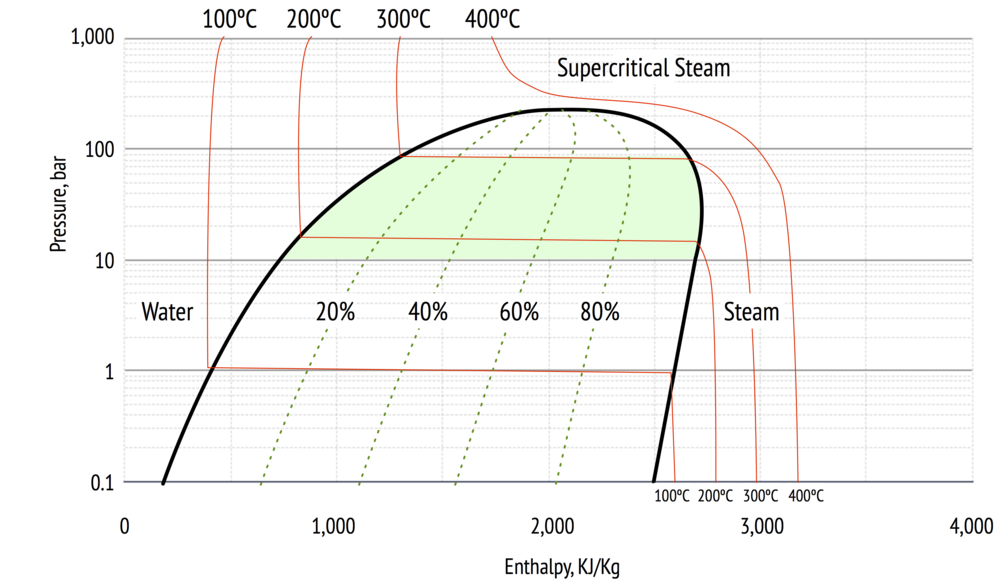
\includegraphics[width=10cm ]{diagramPH.png}
    \caption{P - h diagram}
\end{figure}

With this statement, we see that the terms $h_g(p_1)-h_g(p_2)$ and  $h_l(p_3)-h_l(p_1)$ are very close to zero and, consequently, $Q_{loss}\approx 0$. Finally, we can state that, if the losses are almost zero, the efficiency of the system would be approximately equal to 1.
\section{Gas motion generated by heat}
We can rewrite the expressions for momentum and energy balance (Eq.~\ref{momentum} and Eq.~\ref{energy}) for an ideal gas in a simplified way by combining them with the mass conservation equation (Eq.~\ref{mass}). Let's show the procedure for the momentum equation:
\begin{align}
&(\rho u)_t  + (\rho u u)_x=-p_x\Rightarrow \rho_t u + \rho u_t + (\rho u)_xu+\rho u u_x =-p_x\Rightarrow \nonumber\\
&\Rightarrow - (\rho u)_xu + \rho u_t + (\rho u)_xu+\rho u u_x =-p_x\Rightarrow \rho u_t+\rho u u_x =-p_x
\end{align}
The same procedure will follow with energy conservation. Then, the simplified system is of the form:
\begin{align}
\label{eq:simple_mass}
\rho_t + (\rho u)_{x} =&\ 0,\\
\label{eq:simple_mom}
\rho u_t + \rho u u_x + p_{x} =&\ 0,\\
\label{eq:simple_energ}
\rho c_v T_t - \rho u c_p T_x - \kappa T_{xx} =&\ 0 .
\end{align}
In this section we will study the system in a short time after warming up the gas. Therefore, in order to rescale the system, we will be using the scaling $t=\frac{1}{\epsilon}t$. As the temperature is also dependent on the space, we need to use a different scaling for $x$. A reasonable scale is the parabolic scaling $x=\frac{1}{\sqrt{\epsilon}}x$, as in a duct, the velocity distribution will be subjected to the no-slip condition at the surfaces, while being maximum at the center line. After rescaling, we get the following: 
\begin{align}
\label{eq:scaled_mass}
\frac{1}{\epsilon}\rho_t + \frac{1}{\sqrt{\epsilon}}(\rho u)_{x} =&\ 0,\\
\label{eq:scaled_mom}
\frac{1}{\epsilon}\rho u_t + \frac{1}{\sqrt{\epsilon}}\rho u u_x + p_{x} =&\ 0,\\
\label{eq:scaled_energ}
\frac{1}{\epsilon}\rho c_v T_t - \frac{1}{\sqrt{\epsilon}} \rho u c_p T_x - \frac{1}{\epsilon}\kappa T_{xx} =&\ 0 .
\end{align}
where the scaled variables $t$ and $x$ are of order one.

\section{Two-dimensional model with mass exchange}
Our starting point is the conservation laws for mass and momentum derived above. We assume a stationary case and that the viscous forces dominate. Setting $\lambda = 0$ the equations reduce to:
\begin{align}
\label{eq:momcons}
2\mu \nabla \cdot \varepsilon(u) - \nabla p =&\ 0, \\
\label{eq:masscons}
\nabla (\rho u) =&\ 0,
\end{align}
with $\varepsilon(u) = \frac{1}{2}(\nabla(u) + \nabla(u)^{t})$. We change the notation from $u \in \mathbb{R}^{3}$ to $\textbf{w}(x,y) \in \mathbb{R}^{2}$, with $\textbf{w}(x,y) = u(x,y)\hat{x} + v(x,y)\hat{y}$. Plugging this definition in eq.~\eqref{eq:masscons} gives:
\begin{equation}
\label{eq:masscons2}
(\rho u)_{x} + (\rho v)_{y} = 0.
\end{equation}
We go now to eq.~\eqref{eq:momcons}. Since $\varepsilon$ is a matrix, it is natural to rewrite $\textbf{w}(x,y)$ as:
\begin{equation}
\textbf{w}(x,y) = \begin{pmatrix}
u(x,y) & v(x,y) \\
u(x,y) & v(x,y)
\end{pmatrix}.
\end{equation}
The gradient then is a Jacobian. The matrix $\varepsilon(w)$ then is:
\begin{equation}
\varepsilon(w) = \frac{1}{2}\begin{pmatrix}
2u_{x} & u_{y}+v_x \\
u_{y}+v_x & 2v_{y}
\end{pmatrix}.
\end{equation}
We plug this matrix into eq.~\eqref{eq:momcons} and multiply by the axis vectors $\hat{x} = (1\ 0)$ and $\hat{y} = (0\ 1)$, resulting into the following two equations
\begin{align}
\label{eq:momconsx}
2u_{xx} + u_{yy} + v_{xy} - p_{x} =&\ 0, \\
\label{eq:momconsy}
2v_{yy} + v_{xx} + u_{yx} - p_{y} =&\ 0.
\end{align}
If we now consider an incompressible fluid, i.e. $\rho = constant$, eq.~\eqref{eq:masscons2} then reduces to $u_{x} + v_{y} = 0$ and, by introducing this condition into equations~\eqref{eq:momconsx} and~\eqref{eq:momconsy}, we find the Navier-Stokes equations:
\begin{align}
\label{eq:navmomx}
u_{xx} + u_{yy} - p_{x} =&\ 0,\\
\label{eq:navmomy}
v_{yy} + v_{xx} - p_{y} =&\ 0,\\
\label{eq:navmas}
u_{x} + v_{y} =&\ 0 .
\end{align}
We will now assume incompressibility only for momentum conservation. Our new system is
\begin{align}
\label{eq:navmomx2}
u_{xx} + u_{yy} - p_{x} =&\ 0,\\
\label{eq:navmomy2}
v_{yy} + v_{xx} - p_{y} =&\ 0,\\
\label{eq:navmas2}
(\rho u)_{x} + (\rho v)_{y} =&\ 0 .
\end{align}
The next step is to re-scale these equations. In order to do that, we introduce the variables $\tilde{x} = x$ and $\tilde{y} = \frac{1}{\varepsilon}y$. We then will have $\tilde{u}(\tilde{x},\tilde{y}) = u(\tilde{x},\varepsilon\tilde{y})$ and $\tilde{v}(\tilde{x},\tilde{y}) = v(\tilde{x},\varepsilon\tilde{y})$. By applying the chain rule, we find $u_{xx} = \tilde{u}_{\tilde{x}\tilde{x}}$ and $u_{yy} = \frac{1}{\varepsilon^{2}}\tilde{u}_{\tilde{y}\tilde{y}}$ and similarly for $\tilde{v}(\tilde{x},\tilde{y})$. The system above then reduces to 
\begin{align}
\label{eq:navmomx2sc}
\tilde{u}_{\tilde{x}\tilde{x}} + \frac{1}{\varepsilon^{2}}\tilde{u}_{\tilde{y}\tilde{y}} - \tilde{p}_{\tilde{x}} =&\ 0,\\
\label{eq:navmomy2sc}
\frac{1}{\varepsilon^{2}}\tilde{v}_{\tilde{y}\tilde{y}} + \tilde{v}_{\tilde{x}\tilde{x}} - \frac{1}{\varepsilon}\tilde{p}_{\tilde{y}} =&\ 0,\\
\label{eq:navmas2sc}
\varepsilon(\tilde{\rho} \tilde{u})_{\tilde{x}} + (\tilde{\rho} \tilde{v})_{\tilde{y}} =&\ 0,
\end{align}
with the re-scaled variables $\tilde{p} = \frac{1}{\mu} p$ and $\tilde{\rho}=\frac{1}{\varepsilon}\rho$.\\\\
\textcolor{red}{Before proceeding to solve this system of equations, let us derive the energy conservation equation for \textbf{w}. This will provide an extra condition}\\\\
In the following, we remove the tildes for convenience and simplicity in the notation. Since this system presents a big nonlinear behavior, we will make use of regular perturbation theory in order to solve it. We hence introduces expansions like $f(x,y) \approx f_{0}(x,y) + \varepsilon f_{1}(x,y) + \varepsilon^{2} f_{2}(x,y)+ \dots$ for $u,\ v,\ p,$ and $\rho$. Collecting terms in powers of epsilon, we are left with a system of nine partial differential equations, some of them, coupled:
\begin{align}
\label{eq:diff00}
\mathcal{O}(1)&\left\{\begin{array}{lr}
(u_{0})_{yy} &=\ 0\\
(v_{0})_{yy} &=\ 0\\
(\rho_{0}v_{0})_{y} &=\ 0
  \end{array}\right.\\\nonumber\\
\label{eq:diff01}
  \mathcal{O}(\varepsilon)&\left\{\begin{array}{lr}
  (u_{1})_{yy} &=\ 0\\
  (v_{1})_{yy}+(p_{0})_{y} &=\ 0\\
  (\rho_{0}v_{0})_{x} + (\rho_{0}v_{1})_{y} + (\rho_{1}v_{0})_{y} &=\ 0
    \end{array}\right.\\\nonumber\\
    \label{eq:diff02}
      \mathcal{O}(\varepsilon^{2})&\left\{\begin{array}{lr}
      (u_{0})_{xx}+(u_{2})_{yy}+(p_{0})_{x} &=\ 0\\
     (v_{0})_{xx}+(v_{2})_{yy}+(p_{1})_{y} &=\ 0\\
      (\rho_{0}u_{1})_{x} + (\rho_{1}u_{0})_{y} \\+\ (\rho_{1}v_{1})_{y} + (\rho_{0}v_{2})_{y} + (\rho_{2}v_{0})_{y} &=\ 0
        \end{array}\right.
\end{align}
In order to solve this complex system, we need to set initial and boundary conditions. To do that we look at the following
\begin{figure}[H]
\centering
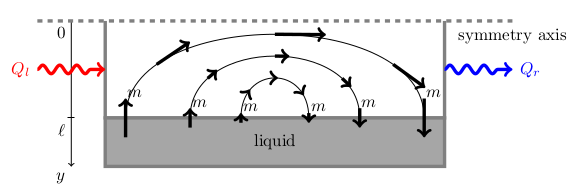
\includegraphics[width=0.7\linewidth]{cosa}
\label{fig:cosa}
\caption{Gas flow with interface mass exchange}
\end{figure}

\noindent By simply looking at figure~\ref{fig:cosa}, we can conclude that there is not vertical component at $y = 0$, which implies \underline{$v(x,0) = 0$}. In addition to this, at $y = 1$ (i.e. $y=l$ scaled), we only find vertical velocity, implying \underline{$u(x,1) = 0$}. We now look at the $x$-component. Since the spatial variables are scaled, we assume that $x \in [0,1]$. At $x=0$ and $x=1$, we again find only vertical component, that is, \underline{$u(0,y) = u(1,y) = 0$}. If we look at $x = \frac{1}{2}$, we see that there is only horizontal component of the velocity, implying \underline{$v(\frac{1}{2},y) = 0$}.
We also assume that the phases are at equilibrium on both ends, implying \underline{$p = p_{sat}(T(x))$}.\\\\
We find more conditions by assuming that there is an underlying flow from left to right as shown in figure~\ref{fig:cosa2}:
\begin{figure}[H]
\centering
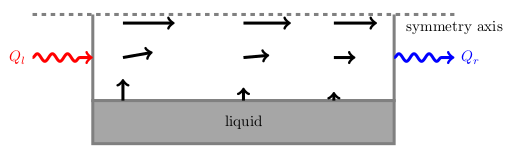
\includegraphics[width=0.7\linewidth]{cosa2}
\caption{Gas flow with interface mass exchange allowing horizontal flow}
\label{fig:cosa2}
\end{figure}

\noindent This simplification shows that at $y=0$, the horizontal component of the velocity is constant in the vertical direction, that is, \underline{$\partial_{y}u(x,0)=0$}. Using this condition and Darcy's approximation, we find \underline{$\partial_{y}p(x,0)=0$}.










\section{Variational part}

I will write this prettier, don't worry ;)

\begin{gather}
    E = E_g+E_s-E_c = 
    \int_0^l \int_0^f(x) \rho g z dz + \alpha (1+f'(x)^2)^\frac{1}{2} dx - \beta f(l) \\
    0 = \delta E = E(f+\delta f)-E(f) = \int_0^l \int_{f(x)}^{f(x)+\delta f} \rho g z dz + \alpha \delta f' \frac{\partial}{\partial f'} (1+f'(x)^2)^\frac{1}{2} dx - \beta \delta f(l) = \\
    \int_0^l \delta f \rho g f(x) + \alpha \delta f' f'(x) (1+f'(x)^2)^{-\frac{1}{2}} dx - \beta \delta f(l) = \\
    \int_0^l \delta f (\rho g f(x) - \alpha f''(x) (1+f'(x)^2)^{-\frac{3}{2}} ) dx + \alpha \Big |_0^l \delta f f'(x) (1+f'(x)^2)^{-\frac{1}{2}} - \beta \delta f(l)\implies \\
    f'(0) = 0 \\
    \alpha f'(l) (1+f'(l)^2)^{-\frac{1}{2}} = \beta \\
    \rho g f(x) = \alpha f''(x) (1+f'(x)^2)^{-\frac{3}{2}}
\end{gather}

\[\Delta p = p_v-p_l\]
\begin{gather}
\delta W_p = \int_0^1 \int_\Omega \Delta p f_\epsilon \  du dv\ d\epsilon = \\
\Delta p \int_0^1 \int_\Omega f_\epsilon\ du dv\ d\epsilon = \\
\Delta p\ \delta V
\end{gather}

\begin{gather}
    A = \int_\Omega (1+f_u^2+f_v^2)^{\frac{1}{2}} du dv \implies \\
    \delta A = \int_0^1 \int_\Omega (f_{u\epsilon}+f_{v\epsilon})(1+f_u^2+f_v^2)^{-\frac{1}{2}} du dv\ d\epsilon \\
    \Delta p \delta V + \sigma \delta A = 0 = \\
    \Delta p \int_0^1 \int_\Omega f_\epsilon\ du dv\ d\epsilon + \sigma \int_0^1 \int_\Omega (f_{u\epsilon}+f_{v\epsilon})(1+f_u^2+f_v^2)^{-\frac{1}{2}} du dv\ d\epsilon = \\
    \int_0^1 \int_\Omega \Delta p f_\epsilon + \sigma (f_{u\epsilon}+f_{v\epsilon})(1+f_u^2+f_v^2)^{-\frac{1}{2}} du dv\ d\epsilon = \\
    \int_0^1 \int_\Omega f_\epsilon (\Delta p  - \sigma (f_{uu}(1+f_v^2)+f_{vv}(1+f_u^2)-2f_{uv} f_u f_v)(1+f_u^2+f_v^2)^{-\frac{3}{2}} du dv\ d\epsilon \implies
\end{gather}
\begin{equation}
\label {Young_Laplace_differential}
    \Delta p  = \sigma (f_{uu}(1+f_v^2)+f_{vv}(1+f_u^2)-2f_{uv} f_u f_v)(1+f_u^2+f_v^2)^{-\frac{3}{2}}
\end{equation}


\begin{gather}
    f(u,v) = \frac{1}{2R_1}u^2+\frac{1}{2R_2}v^2+\text{higher order terms}\\
    f_uu = \frac{1}{R_1}+\text{higher order terms} \\
    f_vv = \frac{1}{R_2}+\text{higher order terms} \\
    \text{Evaluate (\ref{Young_Laplace_differential}) in $u = v = 0$ so higher order terms and $f_u, f_v$ are zero} \\
    \Delta p  = \sigma (f_{uu}+f_{vv}) = \sigma (\frac{1}{R1}+\frac{1}{R2})
\end{gather}

Explanation of 13 a) and 13 b):
Because we are in a stationary state we have $\Delta U = W = 0$, the first law of thermodynamics then gives $Q_{tot} = 0$

$Q_{in}$ and $Q_{out}$ are the heats in and out of the system respectively.
$\kappa_l(T2-T1)$ is the heat transferred through the liquid.
$mh_{lv}$ is the heat going to vaporization / condensation.
$\kappa_v\frac{\partial T}{\partial x}(0)$ and $\kappa_v\frac{\partial T}{\partial x}(L)$ are the heats transferred through the interfaces between vapor and liquid.

\section{Numerical simulation of simplified model}

The equations from \cite{assignment} is like

% Reference section
%\addcontentsline{toc}{section}{References}
\medskip
 
\bibliography{references}

\end{document}
